\documentclass[a4paper,12pt]{article}

\usepackage[utf8]{inputenc}
\usepackage[margin=1in]{geometry}   % page layout
\usepackage{amsmath}                % math
\usepackage{tikz}                   % graphs
\usepackage{tipa}                   % symmbols
\usepackage{indentfirst}            % indents first para of section
\usepackage{color}
\usepackage{listings}

\newcommand{\shrug}[1][]{%
\begin{tikzpicture}[baseline,x=0.8\ht\strutbox,y=0.8\ht\strutbox,line width=0.125ex,#1]
\def\arm{(-2.5,0.95) to (-2,0.95) (-1.9,1) to (-1.5,0) (-1.35,0) to (-0.8,0)};
\draw \arm;
\draw[xscale=-1] \arm;
\def\headpart{(0.6,0) arc[start angle=-40, end angle=40,x radius=0.6,y radius=0.8]};
\draw \headpart;
\draw[xscale=-1] \headpart;
\def\eye{(-0.075,0.15) .. controls (0.02,0) .. (0.075,-0.15)};
\draw[shift={(-0.3,0.8)}] \eye;
\draw[shift={(0,0.85)}] \eye;
% draw mouth
\draw (-0.1,0.2) to [out=15,in=-100] (0.4,0.95); 
\end{tikzpicture}}

\DeclareFixedFont{\ttb}{T1}{txtt}{bx}{n}{12} % for bold
\DeclareFixedFont{\ttm}{T1}{txtt}{m}{n}{12}  % for normal
\definecolor{deepblue}{rgb}{0,0,0.5}
\definecolor{deepred}{rgb}{0.6,0,0}
\definecolor{deepgreen}{rgb}{0,0.5,0}

% Python style for highlighting
\newcommand\pythonstyle{\lstset{
language=Python,
basicstyle=\ttm,
otherkeywords={self},             % Add keywords here
keywordstyle=\ttb\color{deepblue},
emph={MyClass,__init__},          % Custom highlighting
emphstyle=\ttb\color{deepred},    % Custom highlighting style
stringstyle=\color{deepgreen},
frame=tb,                         % Any extra options here
showstringspaces=false            % 
}}

% Python environment
\lstnewenvironment{python}[1][]
{
\pythonstyle
\lstset{#1}
}
{}

\title{LING 23700 Final Project: Emojis \& the Olympics}
\author{Alex Markowitz}
\date{March 16, 2018}

\begin{document}
\maketitle
\tableofcontents
\pagebreak

\section{Introduction}
Since the internet was founded over 40 years ago, language has undergone a revolutionary shift, as online communication becomes an ever-growing percentage of human interaction. As a result, the branch of internet linguistics has been created to analyze and discuss this new form of computer mediated discourse. One specific outcome of the general technological development, and, more recently, the mobile revolution is the introduction of the emoji to our daily lexicon. While the majority of the older generation is opposed to calling these small digital images “language,” most modern linguists agree that emojis are now part of our language and are used to convey additional meaning and tone. Using the 2018 PyeongChang Winter Olympic Games as a lens into global internet linguistics, this paper analyzes data from Twitter to show that while over time, the quantity of available emojis has increased, people remain surprisingly limited with their emoji usage, choosing fewer and happier emojis regardless of their country’s Olympic standing. This points to either a reflection of their expectation for their country’s Olympic performance or an independent relationship between Olympic performance and overall sentiment. 

\subsection{Purpose}
The research question I am interested in pursuing relates to how internet linguistics and computer mediated communication has evolved due to the increase in technology in this millennium. More specifically, I am curious as to how the mobile revolution has shaped communication by looking at the rise of emojis. While some linguists have argued that emojis are a detriment to language, I would like to analyze their effect and support the more recent stance that they do indeed have positive linguistic value.

This project hopes to contribute to the ongoing debate surrounding how emojis impact language. By specifically looking at how emojis are used on Twitter, a social networking site with over 300 million active users, I hope to garner larger insights into their effect on modern day computer mediated communication, proving emojis have benefited modern language by allowing humans to be more expressive over written text; emojis indicate additional expression and feeling behind messages that typed words simply cannot carry. 

I believe this is a valid proposal worth studying because modern technology is omnipresent and becoming increasingly more prevalent in every aspect of our lives. From computers to phones, wearables to “smart” appliances, today’s technology is constantly expanding; it’s important that we stay adaptable as the world around us changes. Understanding how our society interacts with the technology we have created will be crucial in the coming decades as more and more of our lives move online. 

\section{Background}
\subsection{Predecessor to the Emoji}
One recent linguistic phenomenon that came out of the rise of technology has been the use of emoticons. As the immediate predecessor to the emoji, emoticons are simply a combination of ASCII characters used to create an image. Eventually, with the rise in popularity of the internet, and internet messaging specifically, emoticons started to evolve as well. Soon these simple graphics developed into a whole slew of pictorial representations and expanding to include many new objects rather than just faces :-) and emotions $<$3. 

The emoticon evolution only continued its exponential growth in parallel to the rise of mobile phone and specifically, smartphones. With more people having phones that had full keyboards, it was now easier than ever to create more complex emoticons like: \shrug. Starting around 2010, however, emoticons perhaps reached what we can consider their final form of their evolution when they started to be replaced by emojis. While emojis accomplished the same thing, they were actually pictures rather than ASCII characters. 

\subsection{The Emoji}
In the past few years the popularity of emojis has taken off. An emoji keyboard is now included in several mobile operating systems and in 2015, 
\includegraphics[scale=0.035]{faceofjoy.png}, officially called the ‘Face with Tears of Joy’ was named Oxford Dictionary’s Word of the Year. Even within the past year or so, the tech world has now created Bitmojis: “Your own Personal emoji” and Animojis: “custom animated characters…that use your voice and mirror your facial expressions,” which both can claim the simple emoticon as a shared ancestor.

\subsection{Emoji Linguistics}
Due to their immense rise in popularity over the last decade, emojis have been studied and analyzed from a variety of different angles by linguists all over the world, especially those focusing on language of the internet. In his book The Emoji Code, Dr. Vyvyan Evans (2017) explains how emojis hold enough power that they, “can and will be used in a court of law against you.” Wall Street Journal writer Mike Cherney (2018) supports the legitimacy of emojis explaining how many confusing emojis are becoming sources of political and legal debate. However, Emma Reidy (2017) of Emory University explains how emojis easily fit into written language and complement the role of punctuation: “With hilarious and disastrous miscommunications all too common over email and text, emoji may be what conveys the tone and intonation of spoken language.” Internet linguist Gretchen McCulloch (2016) summarizes most modern findings on emojis in that, “they’re trying to solve one of the big problems of writing online, which is that you have the words but you don’t have the tone of voice.” The fact that emojis are studied through these social, legal, and political lenses, lends itself to a highly studied linguistic phenomena with a wide breadth of knowledge upon which to draw various analyses. 

\section{Ethics}
As for the ethical implications of this project, it is important to note that by publishing a tweet on Twitter, the user is agreeing to make that tweet public information. When a user first creates a Twitter account, she is prompted to accept the user policy and therefore is enabling all her further tweets to be accessible by anyone (including users of the Twitter API).

While this is completely legal, one might argue there is a reasonable expectation of privacy – that one’s tweets one signs. However, in this specific case, I do not think users’ tweets regarding the Olympics were to be kept private nor do the tweets contain any kind of information that should remain confidential. Therefore, this project stays within reasonable ethical guidelines.

\section{Data}
Upon completion of the script running, 16,008 tweets were looked at which contained the query “olympics” in them. Of those, 2,493 contained emojis, 1,076 of which were geotagged by country. Portions of the three data maps are attached in Appendix A. 
	
\section{Methods}
To obtain the necessary data, the Twitter API was employed in conjunction with an external Twitter Python library (Tweepy, 2017) while the geolocating of the tweets used the Google Maps Geocoding API. To form my corpus, I used a Python script\footnote{Selected portions in Appendix B} to scrape over 16,000 tweets from Twitter, all containing the phrase “Olympics.” Through the Tweepy library, I was able to efficiently grab 100 tweets at a time containing this phrase and filter out the ones without emojis. Because most tweets regarding the Olympics turned out not to be geotagged, I got location data by looking in the user’s profile of each tweet, and then using the Google Maps API to identify the country of each user. 

The script also imported JSON parsing, printing and data analyzing libraries to assist in producing a concise final report. Through these APIs and libraries, I was able to successfully gather a sufficient corpus needed for analysis.

\section{Analysis}
Upon completion of the script running, the generated report proved to be quite surprising. While these results did help to provide an answer to my question of how emojis are impacting language, they did not directly support my hypothesis as much as I had hoped they would. Based on preliminary research, my hypothesis was that emojis would be a reflection of emotion, closely mirroring the true emotions the original tweeters felt. Thus, those countries that were performing well in the Olympics, relative to the medal count, would use more positive emojis, while countries that were performing poorly, would use a greater amount of negative emojis. 

The biggest surprise of the results was that position in the medal count, or general Olympic performance, had no effect on the degree of positivity of emojis used. When it came to tweeting about the Olympics, everyone was happy; people from all over the globe universally tended to prefer happier emojis in their tweets. Regardless of their position in the medal standings, or even participation in the Olympics at all, the vast majority of countries tended to use many more positive emojis than negative ones. 

Another interesting point of note is that a notable amount of total emojis used were completely neutral. Using the search query of “olympics” prompted the usage of many snowflake, snowing, skiing and snowboarding emojis. While not originally considered, these neutral emojis are not as shocking, as people tend to use emojis to represent things they are discussing, leaving their emotions to the side. 

\section{Conclusion}
Though my hypothesis was unsupported by the data, the findings I gathered reveal a lot of insight into the linguistics of emojis. People overwhelmingly use emojis as a way of expressing happiness rather than expressing the full range of human emotions. Even if people are unpleased with a given topic, they tend to stick to sarcastic emojis before opting for more negative emoji usage. 

To test this, I ran a further analysis of 20,000 tweets with the search query “trump.” While breaking it down on a state-by-state basis did show the expected differences, in terms of liberal states using less positive emojis, the emojis themselves tended to be more sarcastic rather than angry. For example, one of the more popular emojis with this search query was the “face with tears of joy” emoji previously discussed, expressing humor. 

Within the past couple of years there have been many updates to do the emoji lexicon on the main messaging platforms (iOS, Android, Facebook Messenger, etc.) to expand what is possible to be communicated through emojis. However as found in the data, it seems like a majority of people limit their emoji usage into two main groups. Emojis are either being used to express emotion, in which case they more positive, or they are simply used to represent the objects, actions or ideas the rest of the content is referencing. 

\subsection{Future Research \& Greater Picture}
Given the where this project left off, it could possibly be extended to countless different tests. The code written is capable of scraping tens of thousands of tweets in a matter of minutes, with any search query a user chooses and then sorting the results either domestically by state, or internationally by country. 

To gain the most insight it is preferable to use a search query that proves contentious, polarizing the group of people discussing it into various sides. This is why I chose examples from sports and politics, hoping to illicit a stronger divide within my data. 

The next immediate step with the code would be to provide some sort of categorization of emojis – grouping them into positive, neutral and negative emotions to then gather quantifiable insights on their linguistic value. We could then see for example, just which country loves the Olympics the most, or which state thinks President Trump’s actions are most comical. 

In a TED talk video on emoji usage, Dr. Vyvyan Evans uses the example of saying “I love you” lowering his pitch along the way then than saying “I love you” rising his pitch to indicate uncertainty with his statement. He explains how the same phrase can have vastly different meaning and interpretations based on how you say them. Just in the way tone and gestures add meaning to spoken language, emojis are capable of the same thing. Evans (2015) succinctly defines emojis’ role in internet language: “it turns out, that what emoji is doing is fulfilling a function apparent in the spoken channel that’s not there already in the digital channel.”

\subsection{Sources of Error}
While there were no blatant sources of error in the code used, there are a few limitations that constrain my possible results. Both the Twitter and Google Maps APIs limit the amount of requests a user can query in a given time span prohibiting a larger data set from being acquired. Although workarounds exist, to get at least 20,000 tweets, I was hoping to gather data on a much larger scale. 

Additionally, because most tweets are not geotagged with a location by the Twitter user, the only way to get geographical information was to look at the self-reported location of the user profile. The Google Maps API verifies and sorts the real places from the fake but Twitter users use a variety of odd places - from Tatooine to Hogwarts. 

Lastly, it is important to keep in mind the context of the emoji itself. The program strictly limited the data to just emojis rather than the whole content of the tweet. It is very possible that emoji users, albeit a large percentage of total online content creators, are a selective group in that they are a happier set of people. Also, choosing a query of something generally positive, like the Olympics, will naturally illicit positive reactions. 

\pagebreak
\section{Appendix A. Data Mappings}
\subsection{Country Map}
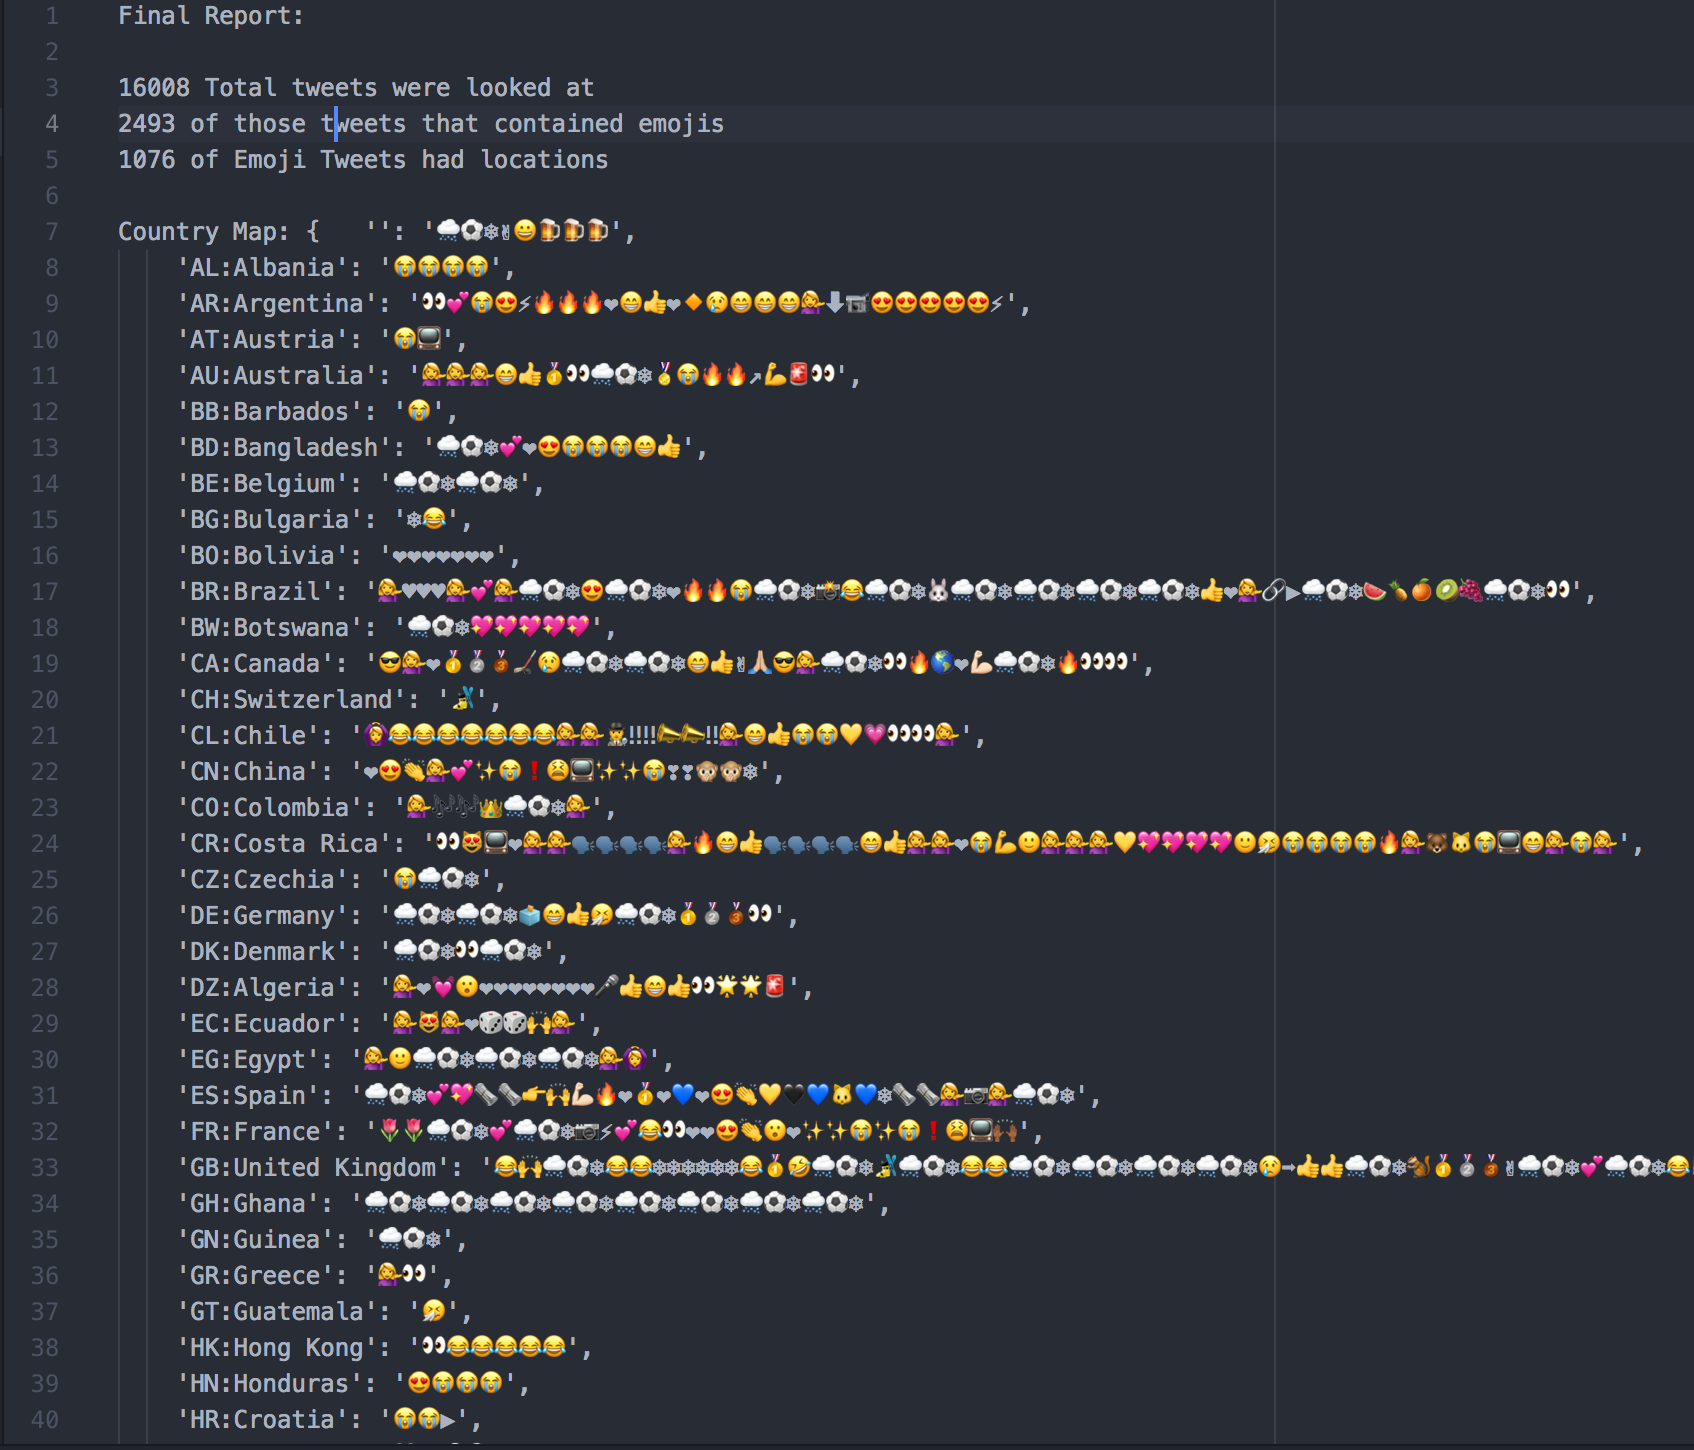
\includegraphics[scale=0.55]{datamap1.png}
\pagebreak
\subsection{Emoji Map}
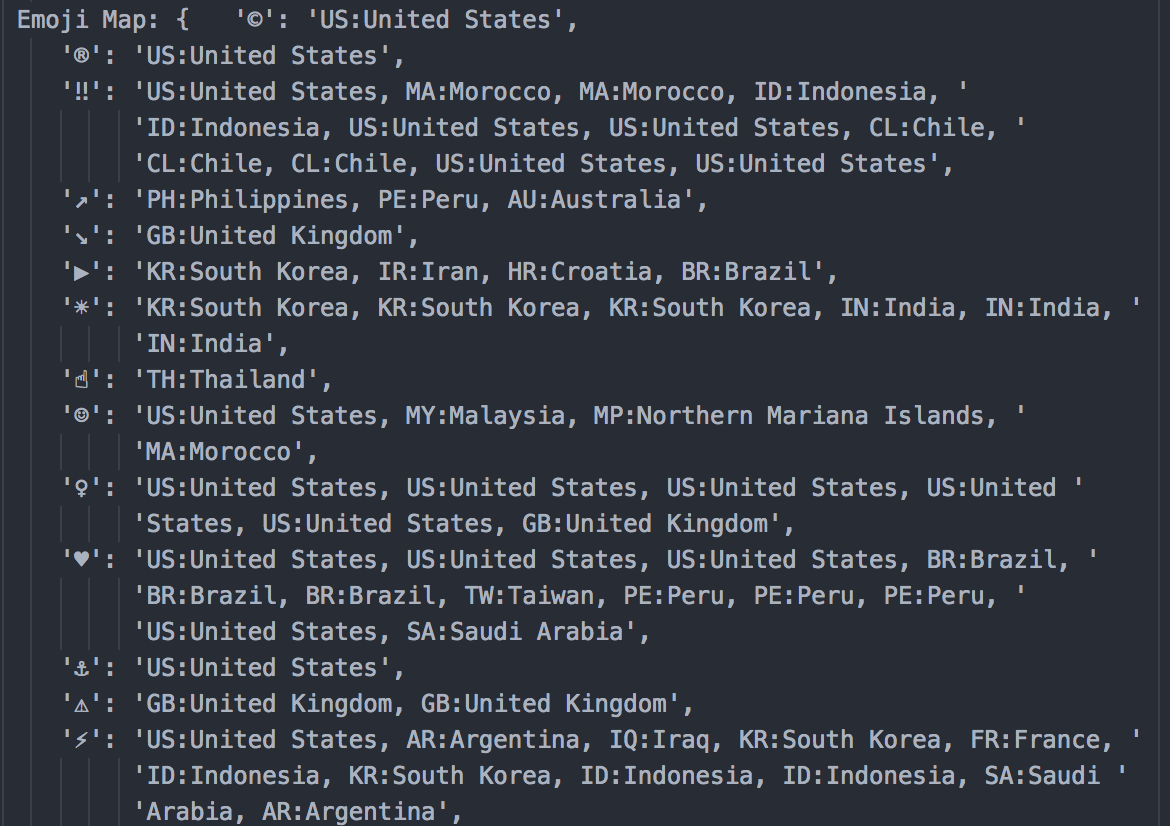
\includegraphics[scale=0.8]{datamap2.png}
\pagebreak
\subsection{Emoji Count}
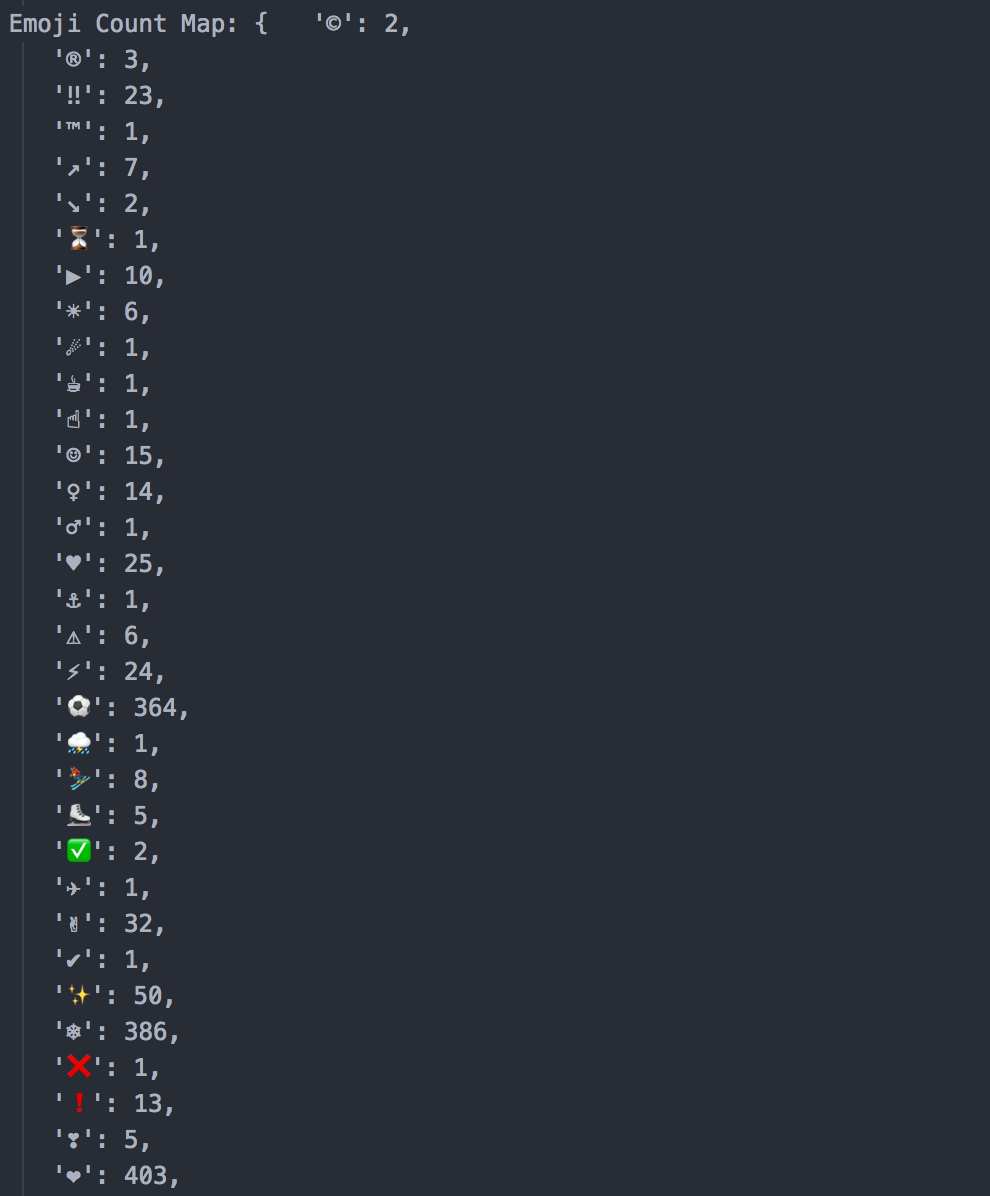
\includegraphics[scale=1.0]{datamap3.png}


\pagebreak
\section{Appendix B. Code}
\begin{python}
# Global Variables
MAX_TWEETS = 20000;
search_query = "olympics";
tweets_per_query = 100;
international = False;          # False searches domestically

emojistat = 0;
stat = 0;
hasLoc = 0;

location_map = {};
emoji_map = {};
emoji_count_map = {};

def getLocation(addr):
    loc = ""
    addCompLen = len(addr)
    for  i in range (0, addCompLen):
        try:
            if international:
                if (addr[i]["types"][0] == "country"):
                    loc += addr[i]["long_name"];
            else:
                if (addr[i]["long_name"] in states):
                    loc += addr[i]["long_name"];
    return loc

def status_has_location(status):
    loc = status.user.location
    if (loc):
        try:
            if (gmaps.geocode(loc)):
                location = getLocation(gmaps.geocode(loc)[0]["address
                _components"])
                if location is not '':
                    insert_location_map(location, status.text);
                    insert_emoji_map(status.text, location);
                    return True;
    else:
        return False;

def insert_location_map(location, status):
    for char in status:
        if(char_is_emoji(char)):
            if location in location_map:
                location_map[location] += char;
            else:
                location_map[location] = char;

def insert_emoji_map(status, location):
    for char in status:
        if(char_is_emoji(char)):
            if char in emoji_map:
                emoji_count_map[char] += 1;
            else:
                emoji_count_map[char] = 1;

            if location is not "none":
                if char in emoji_map:
                    emoji_map[char] += ", {}".format(location);
                else:
                    emoji_map[char] = location;

# loop through MAX_TWEETS tweets to gather data
def main():
    global stat
    global emojistat
    global hasLoc
    
    try:
        if international:
            for status in tqdm(limit_handled(tweepy.Cursor(api.search, 
            q=search_query, count=tweets_per_query).items(MAX_TWEETS))):
                stat += 1
                if(status_has_emoji(status.text)):
                    emojistat += 1;
                    if (status_has_location(status)):
                        hasLoc += 1;
                    else:
                        insert_emoji_map(status.text, "none");
        else:
            for status in tqdm(limit_handled(tweepy.Cursor(api.search, 
            q=search_query, count=tweets_per_query, geocode="39.50,
            -98.35, 1500mi").items(MAX_TWEETS))):
                stat += 1
                if(status_has_emoji(status.text)):
                    emojistat += 1;
                    if (status_has_location(status)):
                        hasLoc += 1;
                    else:
                        insert_emoji_map(status.text, "none");
    report(stat, emojistat, hasLoc);

main();
\end{python}

\pagebreak
\section{Bibliography}
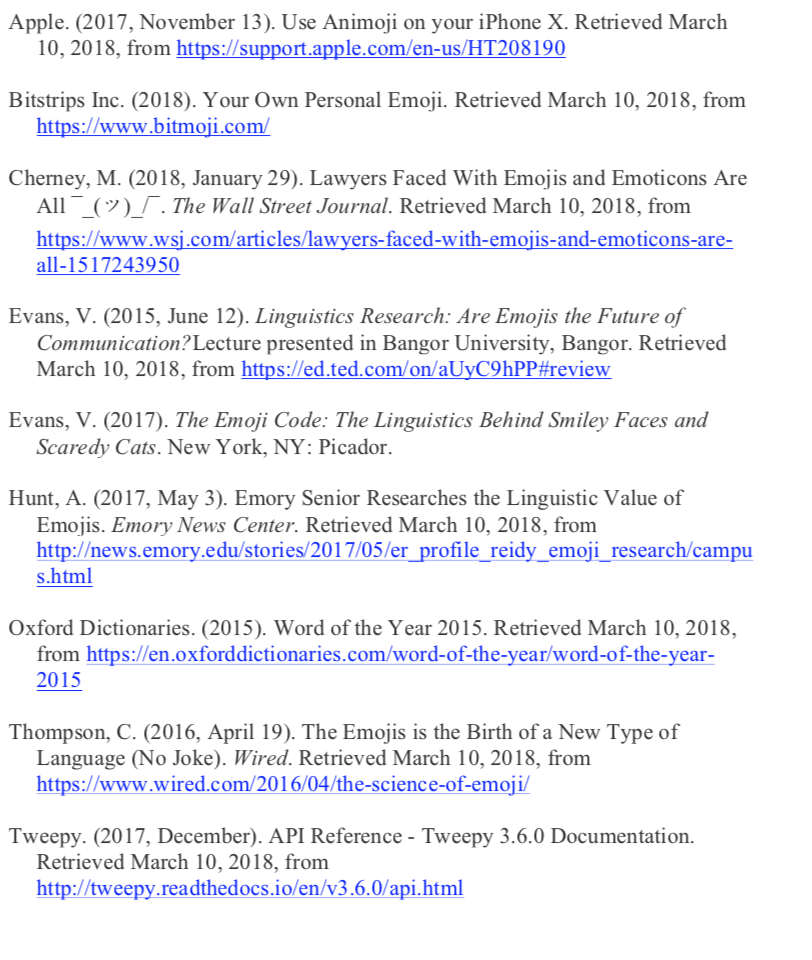
\includegraphics[scale=1.1]{bib.png}



\end{document}
